\section{Experiments}

\subsection{Benchmarks}

We evaluate our models across six diverse benchmarks spanning mathematics and code generation. 
Each dataset targets a different aspect of reasoning or problem-solving: 
(1) \textbf{AIME 24} is an annual high-school mathematics competition from the American Mathematics Competitions (AMC) series. The 2024 set contains 30 problems designed to test advanced mathematical reasoning, covering algebra, number theory, geometry, and combinatorics;
(2) \textbf{AIME 25} is the 2025 edition of the AIME competition, with a new set of 30 problems of comparable style and difficulty;
(3) \textbf{HMMT Feb 25} is a premier international high-school mathematics tournament. We evaluate on the February 2025 contest set, which contains 30 problems spanning diverse mathematical domains;
(4) \textbf{LiveCodeBench v5 (2408–2502)} \citep{jain2024livecodebench} is a live-updated benchmark that sources real-world coding problems from LeetCode, AtCoder, and CodeForces. We use the problems released between August 2024 and February 2025, totaling 279 problems;
(5) \textbf{LiveCodeBench v6 (2502–2505)}~\citep{jain2024livecodebench} extends the dataset with newer problems released between February 2025 and May 2025, containing 131 problems. This split highlights temporal generalization by evaluating on problems unseen in v5;
and (6) \textbf{Codeforces}~\citep{quan2025codeelo} consists of 408 real-world competitive programming problems drawn from the Codeforces platform. Problems cover a wide spectrum of algorithmic reasoning challenges and reflect authentic conditions faced in live contests.  

\subsection{Evaluation Metrics}

We adopt \textbf{pass@1 accuracy} as the primary evaluation metric across all benchmarks. 
For mathematical benchmarks (AIME 24, AIME 25, HMMT Feb 25), we report \textbf{avg@16}, where pass@1 accuracy is averaged over 16 independent generations per problem to reduce evaluation variance. 
For programming benchmarks (LiveCodeBench v5, LiveCodeBench v6), we report the standard \textbf{pass@1}, computed from a single generation per problem. 
In both cases, correctness is determined strictly: a mathematical output must exactly match the ground-truth final boxed answer, while a programming output must pass all provided functional unit tests. 

For the Codeforces benchmark, we follow the evaluation protocol of \citet{luo2025deepcoder} and compute Elo ratings to evaluate the performance gap between models and competitive programming experts.
Each problem is attempted with up to 8 independent generations, and the Elo system aggregates outcomes to produce a competitive programming–style performance measure.  

\subsection{Baselines}

We evaluate against two complementary experimental settings: \emph{self-play} and \emph{SFT}. 
Both settings rely on the same family of problem curation baselines, but differ in base models and in how the released corpora are utilized.

\paragraph{Self-Play.}
We compared PromptCoT~2.0 against a set of open-source corpora comprising large-scale mathematical and programming problems, as well as mixed collections. Prompts from each corpus were used to train \texttt{Qwen3-4B-Thinking-2507} and \texttt{Qwen3-30B-A3B-Thinking-2507}~\citep{yang2025qwen3} under the self-play setting. Specifically, we considered the following corpora:
(1) \textbf{OpenCodeReasoning}~\citep{ahmad2025opencodereasoning}, containing curated competitive programming problems from Codeforces, AtCoder, and LeetCode;
(2) \textbf{OpenMathReasoning}~\citep{moshkov2025aimo}, consisting of competition-style mathematics problems from AoPS and related repositories;
(3) \textbf{OpenThoughts3}~\citep{guha2025openthoughts}, a collection of curated cross-domain questions augmented with synthetic generation;
(4) \textbf{OpenR1}~\citep{openr1}, comprising curated problems from Codeforces and NuminaMath variants; and
(5) \textbf{PromptCoT~1.0}~\citep{zhao2025promptcot,zhao2025scaling}, a corpus of mathematics and programming problems augmented through the concept–rationale–prompt paradigm. Since the original corpora were designed for large-scale SFT and were therefore too large for self-play, we downsampled their prompt sets to ensure all methods operated on comparable data sizes.






\paragraph{SFT.} The base model used is \texttt{Qwen2.5-7B-Instruct}~\citep{yang2024qwen2_5}. For PromptCoT~1.0, we adhered to the training protocol outlined in \citet{zhao2025scaling}. For the other baselines, we directly evaluated the officially released checkpoints without any additional training or modifications. In addition, we included an \textbf{OpenThoughts3 (GPT)} variant, where the prompts are identical to those of OpenThoughts3 but the responses are generated using \texttt{GPT-OSS-120B (medium)}, allowing a controlled comparison with our method.



\begin{table}[t]
\centering
\resizebox{0.9\textwidth}{!}{
\begin{tabular}{lcccccc}
\toprule
\textbf{Model} & \textbf{AIME 24} & \textbf{AIME 25} & \textbf{HMMT Feb 25} & \makecell{\textbf{LiveCodeBench v5} \\ \textbf{(2408--2502)}} & \makecell{\textbf{LiveCodeBench v6} \\ \textbf{(2502--2505)}} & \textbf{Codeforces} \\
\midrule
\textbf{Qwen3-4B-Thinking-2507} & 85.2 & 81.3 & 55.5 & 63.8 & 55.2 & 1852 \\ \midrule
\textbf{OpenCodeReasoning}      & 83.1 & 78.5 & 50.4 & 64.4 & \underline{57.1} & 1867 \\
\textbf{OpenMathReasoning}      & \underline{85.3} & \underline{83.0} & 56.8 & 59.7 & 48.5 & 1826 \\
\textbf{OpenThoughts3}          & 84.7 & 80.6 & 54.2 & \underline{65.2} & 54.4 & 1846 \\
\textbf{OpenR1}                 & 84.6 & 80.9 & 56.7 & 63.0 & 54.6 & 1829 \\
\textbf{PromptCoT 1.0}          & \underline{85.3} & 81.8 & \underline{58.6} & 64.5 & 56.7 & \underline{1878} \\ \midrule
\textbf{PromptCoT 2.0}          & \textbf{87.3} & \textbf{85.0} & \textbf{66.5} & \textbf{67.7} & \textbf{61.1} & \textbf{1934} \\
\bottomrule
\end{tabular}
}
\caption{Evaluation results on six benchmarks under the Self-Play setting using models with \textbf{4B} parameters. Bold values denote the best performance for each benchmark, while underlined values denote the second-best.}
\label{tab:baselines-4b}
\end{table}


\begin{table}[t]
\centering
\resizebox{0.9\textwidth}{!}{
\begin{tabular}{lcccccc}
\toprule
\textbf{Model} & \textbf{AIME 24} & \textbf{AIME 25} & \textbf{HMMT Feb 25} & \makecell{\textbf{LiveCodeBench v5} \\ \textbf{(2408--2502)}} & \makecell{\textbf{LiveCodeBench v6} \\ \textbf{(2502--2505)}} & \textbf{Codeforces} \\
\midrule
\textbf{Qwen3-30B-A3B-Thinking-2507} & 87.7 & 85.0 & 71.4 & 68.1 & 66.0 & 2044 \\ \midrule
\textbf{OpenCodeReasoning}       & 85.0 & 81.1 & 64.9 & \underline{70.8} & 67.4 & 2048 \\
\textbf{OpenMathReasoning}       & \underline{87.9} & 86.1 & \underline{72.2} & 65.7 & 58.4 & 2022 \\
\textbf{OpenThoughts3}           & 85.7 & 84.7 & 70.0 & 68.3 & 67.2 & 2019 \\
\textbf{OpenR1}                  & 86.3 & 84.9 & 68.9 & 68.3 & 63.7 & 2045 \\
\textbf{PromptCoT 1.0}           & 86.8 & \underline{87.4} & 72.0 & 69.7 & \underline{67.8} & \underline{2051} \\ 
\midrule
\textbf{PromptCoT 2.0}           & \textbf{92.1} & \textbf{89.8} & \textbf{76.7} & \textbf{74.2} & \textbf{71.0} & \textbf{2079} \\
\bottomrule
\end{tabular}
}
\caption{Evaluation results on six benchmarks under the Self-Play setting using models with \textbf{30B-A3B} parameters. Bold values denote the best performance for each benchmark, while underlined values denote the second-best.}
\label{tab:baselines-30b}
\end{table}

\begin{table}[t]
\centering
\resizebox{1.0\textwidth}{!}{
\begin{tabular}{lcccccccccc}
\toprule
\textbf{Model} & \textbf{Prompt Source} & \textbf{Teacher Model} & \textbf{Dataset Size} & \textbf{Avg. Resp. Len.} & \textbf{AIME 24} & \textbf{AIME 25} & \textbf{HMMT Feb 25} & \makecell{\textbf{LCB v5} \\ \textbf{(2408--2502)}} & \makecell{\textbf{LCB v6} \\ \textbf{(2502--2505)}} & \textbf{Codeforces} \\
\midrule
\textbf{Qwen2.5-7B-Instruct} & - & - & - & - & 12.8 & 8.0 & 2.7 & 14.7 & 13.7 & 706 \\ \midrule
\textbf{OpenCodeReasoning} & H & DeepSeek-R1 & 0.75M & 12878.9 & 11.7 & 7.7 & 6.0 & \underline{50.5} &  42.0 & \underline{1648} \\
\textbf{OpenMathReasoning} & H & DeepSeek-R1 & 4.92M & 14407.5 & \textbf{73.3} & 58.1 & \underline{42.1} & 9.7 & 10.7 & 676 \\
\textbf{OpenThoughts3} & H+S & QwQ-32B & 1.20M & 18740.2 & 69.6 & 59.4 & 38.3 & 47.0 & 36.6 & 1630 \\
\textbf{OpenR1} & H & DeepSeek-R1 & 0.35M & 14974.3 & 55.6 & 39.2 & 24.6 & 40.5 & 32.8 & 1548 \\
\textbf{PromptCoT 1.0} & H+S & QwQ-32B & 1.25M & 16323.5 & 71.0 & \underline{60.2} & 41.6 & 47.8 & \underline{43.6} & 1645 \\ 
\textbf{OpenThoughts3 (GPT)} & H+S & \makecell{GPT-OSS-120B \\ (medium)} & 1.20M & 8967.2 & 52.3 & 37.3 & 24.0 & 22.2 & 21.4 & 907 \\ \midrule
\textbf{PromptCoT 2.0} & S & \makecell{GPT-OSS-120B \\ (medium)} & 4.77M & 7351.2 & \underline{73.1} & \textbf{65.6} & \textbf{46.5} & \textbf{53.4} & \textbf{48.9} & \textbf{1815} \\
\bottomrule
\end{tabular}
}
\caption{Evaluation results on six benchmarks under the SFT setting using models with \textbf{7B} parameters. 
\textbf{H} = Human-written, \textbf{S} = Synthetic, \textbf{Avg. Resp. Len.} = average response length, and \textbf{LCB} = LiveCodeBench. 
Bold values denote the best performance for each benchmark, while underlined values denote the second-best.}
\label{tab:baselines-7b}
\end{table}




\subsection{Implementation Details}

\subsubsection{Prompt Synthesis}

\paragraph{Code-start Initialization.} 
We initialized the framework using open-source problem collections, drawing 9,221 programming problems from Codeforces~\citep{penedo2025codeforces} and 6,365 mathematics problems from AoPS\footnote{\url{https://artofproblemsolving.com/}}. 
For each problem, we annotated associated concepts and rationales by querying four high-capacity instruction-tuned models: \texttt{Qwen2.5-32B-Instruct}, \texttt{Qwen2.5-72B-Instruct}, \texttt{Llama-3.1-70B-Instruct}~\citep{grattafiori2024llama} and \texttt{phi-4}~\citep{abdin2024phi}. 
The instructions used for concept extraction and rationale generation are provided in Appendix~\ref{app:concept_prompt} and Appendix~\ref{app:rationale_prompt}, respectively.
These annotations provided the supervision to warm-start both the rationale generation model and the prompt generation model, both of which were initialized from \texttt{Qwen2.5-32B-Base}. 
Models were trained with a learning rate of $2 \times 10^{-5}$, a batch size of 16, and for two epochs. 



\paragraph{EM Optimization.} 
In the EM refinement stage, the rationale generation model (E-step) was trained with a learning rate of $2 \times 10^{-6}$, a batch size of 16, and a sampling temperature of 1.0.  
% For each concept–prompt pair, we sampled eight candidate rationales and selected the one achieving the highest reward to update the model parameters.  
In the M-step, rationales decoded deterministically from this model (temperature 0.0) were used to update the prompt generation model, which was trained with a learning rate of $2 \times 10^{-6}$ and a batch size of 16.  


\subsubsection{Post-training with Synthesized Prompts}
\label{sec:details_post_train}
\paragraph{Self-Play.} 
For the 4B models, we constructed a training corpus of 48,113 prompts, comprising 4,707 programming prompts and 43,406 mathematics prompts. 
Among the programming prompts, 1,872 were synthesized using PromptCoT~2.0, while 2,835 were drawn from Codeforces~\citep{penedo2025codeforces} and LiveCodeBench contest problems released prior to August 2024. 
For mathematics, 30,435 prompts were synthesized using PromptCoT~2.0 and 12,971 originate from DeepScaleR~\citep{deepscaler2025}. 
Each synthesized programming prompt was paired with 3–4 automatically generated unit tests using \texttt{Qwen3-32B}, while each synthesized mathematics prompt was paired with a final boxed answer obtained via majority voting over 8 generations from \texttt{Qwen3-30B-A3B-2507-Thinking}.

For the 30B-A3B models, we prepared a dataset of 11,209 prompts, including 3,072 programming prompts and 8,137 mathematics prompts. 
Within programming, 1,024 prompts were synthesized using PromptCoT~2.0 and 2,048 came from Codeforces and LiveCodeBench problems (prior to August 2024). 
In mathematics, 3,333 prompts were synthesized using PromptCoT~2.0 and 4,804 were sourced from DeepScaleR. 
Similarly, synthesized programming prompts were paired with 3–4 unit tests generated by \texttt{Qwen3-32B}, while mathematics prompts were paired with final boxed answers determined through majority voting over 8 generations from \texttt{GPT-OSS-120B (medium)}.

During self-play, we use a binary reward $u(x,y)$: $u(x,y)=1$ if (i) the generated final answer exactly matches the boxed reference for mathematics, or (ii) the generated program passes all unit tests for programming; otherwise $u(x,y)=0$. 
Self-play training was conducted with direct preference optimization (DPO)~\citep{rafailov2023direct}.  
For each prompt $x$, we sampled eight rollouts and evaluated them using the reward $u(x,y)$.  
Rollouts with $u(x,y)=1$ were treated as positive samples, while those with $u(x,y)=0$ were treated as negative samples.  
To ensure adequate task difficulty, we applied a filtering step: problems that the self-play models solved in at least half of eight independent attempts were excluded. 
Sampling temperatures were set to 1.25 for 4B models and 1.2 for 30B-A3B models respectively, as higher temperatures were found to substantially increase the proportion of invalid rollouts (e.g., formatting errors or corrupted outputs). 
Potential overlap with evaluation sets was mitigated by 13-gram matching to remove contaminated instances~\citep{yang2024qwen2_5}. 
All self-play training runs used a batch size of 16 and a learning rate of $1 \times 10^{-6}$. 

\paragraph{SFT.}
For the SFT setting, we employed \texttt{GPT-OSS-120B (medium)} as the teacher model. 
All training prompts were synthesized using PromptCoT~2.0, \textit{without} incorporating external problem collections. 
We applied a light filtering step, discarding instances where the teacher failed to produce a valid final boxed answer (for mathematics) or an executable code snippet (for programming). 
This process produced a corpus of 4,766,890 prompts, consisting of 1,188,505 programming prompts and 3,578,385 mathematics prompts. 
Training was performed with a batch size of 1,024 and a learning rate of $8 \times 10^{-5}$.




\subsection{Main Results}
\paragraph{Self-Play Setting.}
Table~\ref{tab:baselines-4b} and Table~\ref{tab:baselines-30b} report the results of self-play experiments, from which several noteworthy observations emerge: (1) Incorporating rationales proves beneficial for synthesizing high-quality prompts, even when implemented in a straightforward manner through prompt engineering (i.e., PromptCoT~1.0). 
(2) PromptCoT~2.0 exhibits superior data efficiency: in the 4B setting, it attains superior results using only about 90\% of the math prompts and 10\% of the code prompts compared to OpenMathReasoning and OpenCodeReasoning. The 30B setting further reduces the required data while achieving even stronger gains.
(3) While both OpenThoughts3 and OpenR1 include a substantial proportion of high-quality, human-crafted mathematics and programming questions, they generally fail to provide further gains for strong models such as \texttt{Qwen3-4B-Thinking-2507} and \texttt{Qwen3-30B-A3B-Thinking-2507}. A plausible explanation is that such data may have already been incorporated into the training of these models. In contrast, despite the already strong capabilities of the base models, prompts synthesized by PromptCoT~2.0 deliver consistent and significant improvements across a wide range of mathematical and programming tasks, underscoring the considerable potential of prompt synthesis in advancing the frontier of reasoning LLMs. (4) Finally, the advantage of PromptCoT~2.0 over the baseline methods becomes even more pronounced on challenging tasks such as HMMT, a gain that can be attributed to its EM-based rationale generation, which provides stronger inductive signals for synthesizing sufficiently difficult questions for these benchmarks.

\paragraph{SFT Setting.}
We further evaluate PromptCoT~2.0 under the SFT setting, with results presented in Table~\ref{tab:baselines-7b}. From the results, we draw several key observations: (1) With 100\% synthesized prompts, PromptCoT~2.0 delivers strong performance across all benchmarks. Given that prompt synthesis is far more scalable than manual curation, these results highlight the considerable potential of scaling synthetic data for future advances in LLM reasoning. (2) Beyond its superior performance, the dataset produced by PromptCoT~2.0 also exhibits substantially shorter reasoning traces, leading to notable computational savings during inference. While this property may largely stem from the teacher model, the released dataset—owing to its scale, quality, and compact responses—stands to provide significant benefit to the broader community.







\begin{table}[t]
\centering
\resizebox{0.9\textwidth}{!}{
\begin{tabular}{lcccccc}
\toprule
\textbf{Model Variant} & \textbf{AIME 24} & \textbf{AIME 25} & \textbf{HMMT Feb 25} & \makecell{\textbf{LiveCodeBench v5} \\ \textbf{(2408--2502)}} & \makecell{\textbf{LiveCodeBench v6} \\ \textbf{(2502--2505)}} & \textbf{Codeforces} \\
\midrule
\textbf{PromptCoT 2.0 (full)} & \textbf{73.1} & \textbf{65.6} & \textbf{46.5} & \textbf{53.4} & \textbf{48.9} & \textbf{1815} \\ \midrule
\quad -- Code-start            & 72.1 & 63.9 & 45.3 & 50.4 & 43.6 & 1677 \\
\quad -- EM                    & 69.8 & 59.0 & 41.3 & 44.9 & 44.2 & 1592 \\
\bottomrule
\end{tabular}
}
\caption{Ablation results under the SFT setting using models with \textbf{7B} parameters. Bold numbers indicate the highest performance.}
\label{tab:ablation}
\end{table}


\subsection{Ablation Study}

We conducted an ablation study under the SFT setting using 7B models to evaluate the contribution of each component in PromptCoT~2.0. Specifically, we considered two variants: (1) removal of the cold-start stage, denoted as ``- Code-start''; and (2) removal of the EM optimization stage, denoted as ``- EM''. The results are summarized in Table~\ref{tab:ablation}.

The full PromptCoT~2.0 consistently outperforms both ablated variants across all six benchmarks, underscoring the necessity of both stages. Excluding the cold-start stage leads to a moderate but consistent performance decline, showing that high-quality initial annotations from large teacher models are essential for stabilizing the subsequent training loop. In contrast, removing the EM optimization stage causes the largest performance drop, particularly on HMMT and Codeforces, demonstrating that the iterative refinement of rationales and prompts is central to the success of our approach.



\begin{figure}[t]
    \centering
    % First row
    \begin{subfigure}{0.48\textwidth}
        \centering
        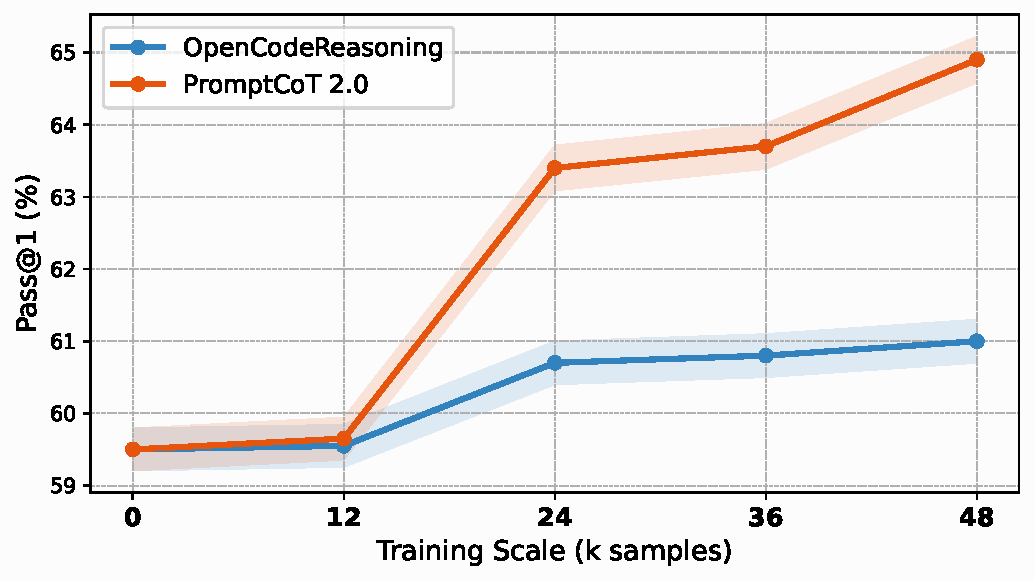
\includegraphics[width=\linewidth]{selfplay_code.pdf}
        \caption{Self-play on code benchmarks.}
    \end{subfigure}
    \hfill
    \begin{subfigure}{0.48\textwidth}
        \centering
        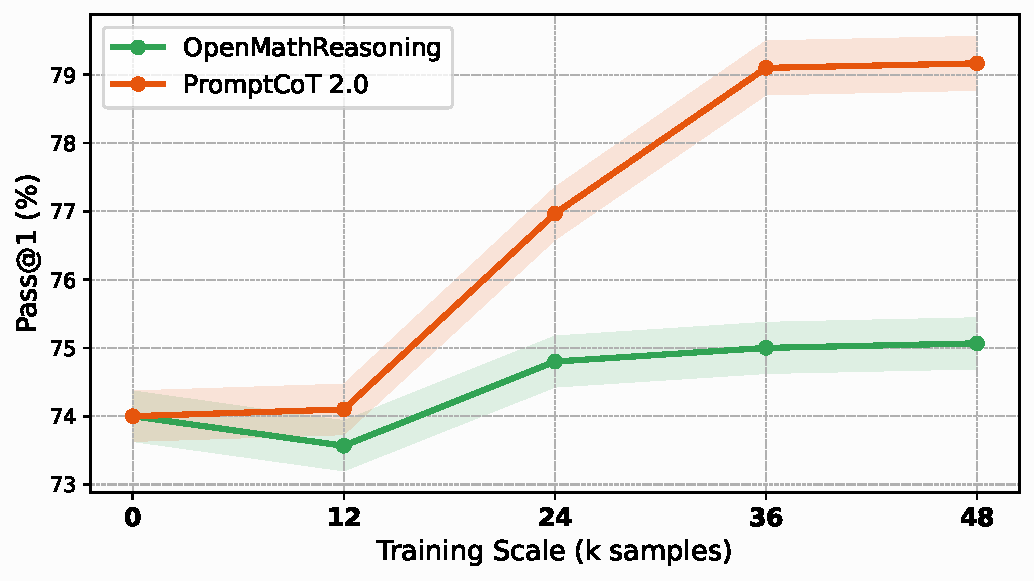
\includegraphics[width=\linewidth]{selfplay_math.pdf}
        \caption{Self-play on math benchmarks.}
    \end{subfigure}

    % Second row
    \vspace{0.4em}
    \begin{subfigure}{0.48\textwidth}
        \centering
        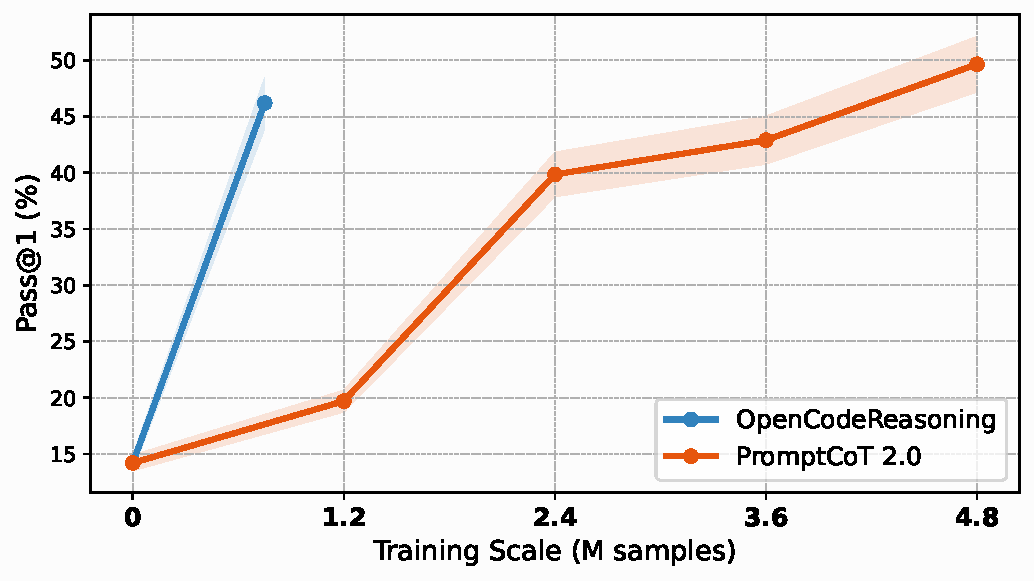
\includegraphics[width=\linewidth]{sft_code.pdf}
        \caption{SFT on code benchmarks.}
    \end{subfigure}
    \hfill
    \begin{subfigure}{0.48\textwidth}
        \centering
        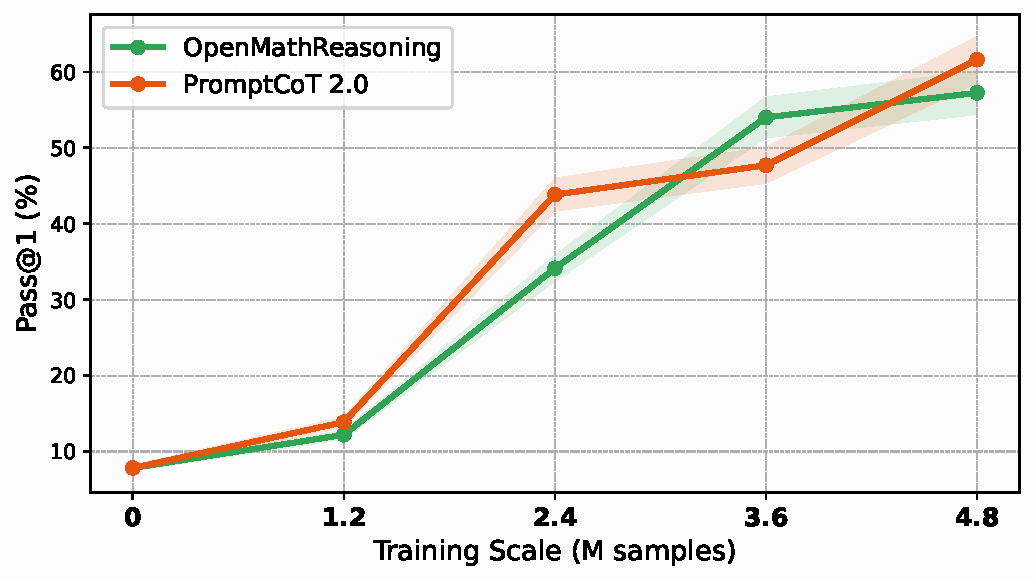
\includegraphics[width=\linewidth]{sft_math.pdf}
        \caption{SFT on math benchmarks.}
    \end{subfigure}

    \caption{Learning curves of PromptCoT~2.0 compared with baseline methods.}
    \label{fig:learning_curves}
\end{figure}


\subsection{Scaling Properties}
\label{sec:scaling}

We next examined the scaling behavior of PromptCoT~2.0 compared to curation-based baselines under both the self-play and the SFT settings.  
For self-play experiments, we initialized from \texttt{Qwen3-4B-Thinking-2507} and progressively increase the number of training examples.  
For SFT experiments, we initialized from \texttt{Qwen2.5-7B-Instruct}, again varying the amount of training data.  
To ensure comparability, we randomly sampled each dataset to match the desired scale.  
We report results on mathematics and programming benchmarks separately, and in all cases we plot the average accuracy across the relevant benchmarks (AIME~24, AIME~25, HMMT~Feb~25 for mathematics; LiveCodeBench v5 and v6 for programming).  

\paragraph{Self-play scaling.}  
Figure~\ref{fig:learning_curves} (a) and Figure~\ref{fig:learning_curves} (b) illustrate the effect of increasing training examples from 0 to 48k.  
The curation-based baselines show limited or even unstable improvements, with performance gains largely saturating beyond 24k examples.  
In contrast, PromptCoT~2.0 demonstrates consistent scaling: accuracy steadily improves with additional data.  
This highlights the advantage of EM-guided rationale–prompt synthesis, which produces higher-quality problems that continue to yield benefits at larger scales.  

\paragraph{SFT scaling.}  
Figure~\ref{fig:learning_curves} (c) and Figure~\ref{fig:learning_curves} (d) report the effect of increasing training data size from 0 to 4.8M examples.  
Here too, the difference between curation-based and rationale-driven synthesis is pronounced.  
While baselines exhibit sharp but plateauing gains, PromptCoT~2.0 achieves both higher peak performance and stronger data efficiency.  




\begin{figure}[t]
    \centering
    % Left: Code MDS
    \begin{subfigure}{0.48\textwidth}
        \centering
        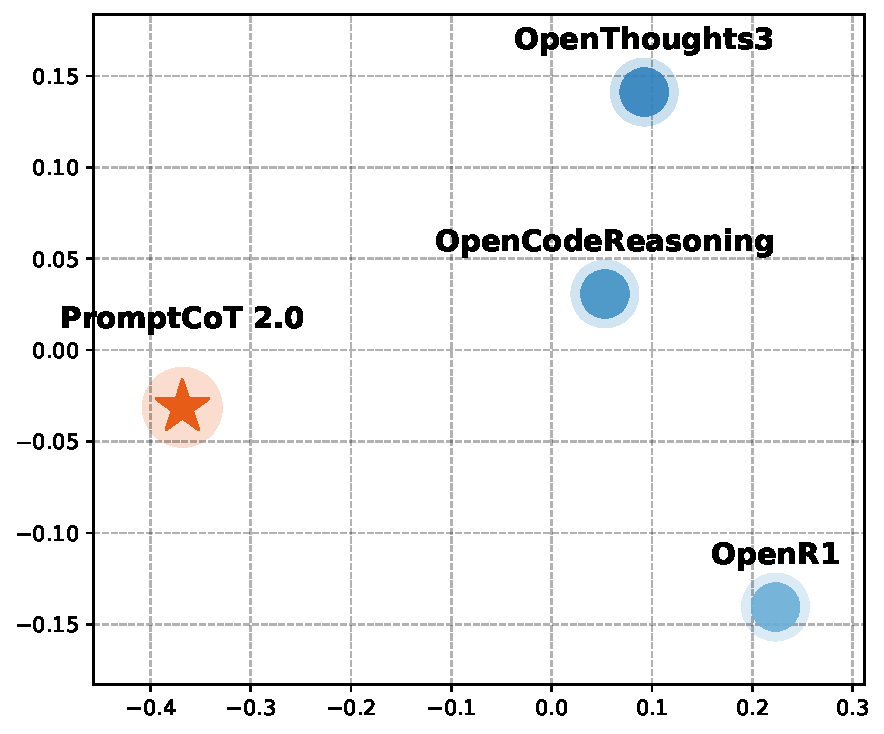
\includegraphics[width=\linewidth]{code_mds.pdf}
        \caption{MDS visualization for code datasets.}
    \end{subfigure}
    \hfill
    % Right: Math MDS
    \begin{subfigure}{0.48\textwidth}
        \centering
        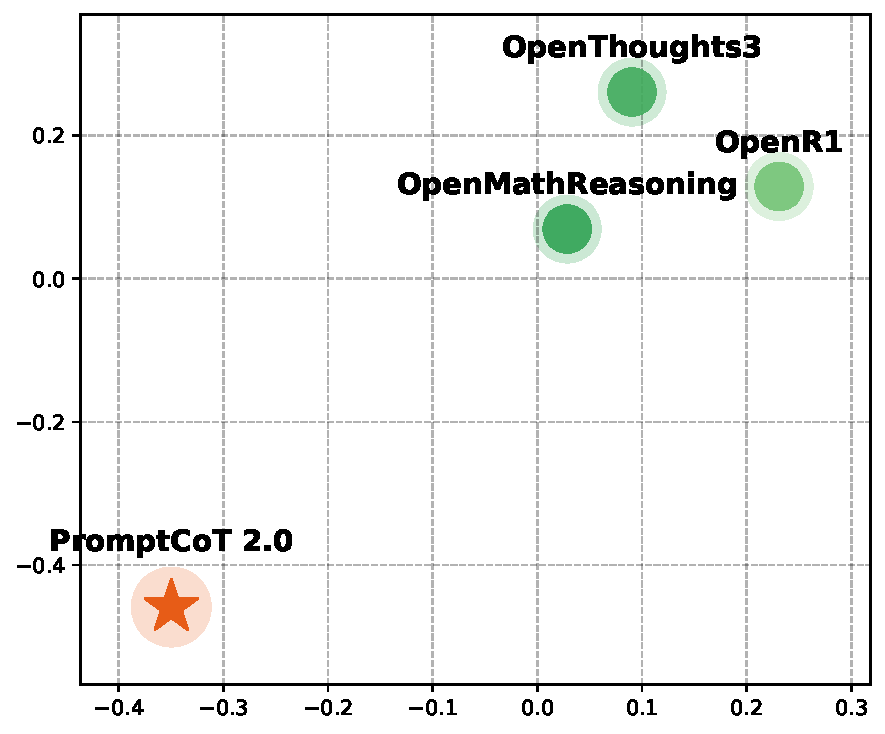
\includegraphics[width=\linewidth]{math_mds.pdf}
        \caption{MDS visualization for math datasets.}
    \end{subfigure}

    \caption{Multidimensional scaling (MDS) projections of dataset-level embeddings.
    Distances are based on cosine dissimilarity between average problem embeddings.}
    \label{fig:dataset_mds}
\end{figure}


\subsection{Distributional Analysis}
\label{sec:distributional_analysis}

To investigated the distributional properties of our synthesized problems relative to existing open-source datasets, we computed embeddings for each problem using the \texttt{all-MiniLM-L6-v2} sentence transformer~\citep{wang2020minilm}.  
For each dataset, we took the average embedding across all problems to obtain a dataset-level representation.  
Pairwise distances were then computed as $d(A, B) = 1 - \mathrm{cos}(A, B)$, where $\mathrm{cos}(\cdot, \cdot)$ denotes cosine similarity.  
We applied multidimensional scaling (MDS) to project these distances into two dimensions, yielding a visualization that captures relative relationships among datasets in a low-dimensional space.

The results, shown in Figure~\ref{fig:dataset_mds}, reveal two notable findings:  
(1) Existing open-source datasets (e.g., OpenCodeReasoning, OpenMathReasoning, OpenThoughts3, and OpenR1) form tight clusters, reflecting their high similarity and shared reliance on either curated or slightly varied synthetic problems.  
(2) In contrast, our synthesized problems (\textsc{PromptCoT~2.0}) occupy a distinct region in the embedding space, indicating substantial distributional differences from existing corpora. This separation suggests that our rationale-driven synthesis paradigm not only generates problems at scale, but also introduces novel linguistic and structural variations beyond the scope of prior datasets.  


\begin{table}[t]
\centering
\resizebox{0.65\textwidth}{!}{
\begin{tabular}{lcc}
\toprule
\textbf{Dataset} & \makecell{\textbf{Qwen2.5-72B-Instruct} \\ \textbf{Accuracy} ($\downarrow$)} & 
\makecell{\textbf{GPT-OSS-120B (high)} \\ \textbf{Avg. Resp. Tokens} ($\uparrow$)} \\
\midrule
\textbf{OpenMathReasoning}$^\dagger$ & 28.9 & 18,436.9 \\
\textbf{OpenThoughts3}$^\dagger$     & 21.3 & 30,053.7 \\
\textbf{OpenR1}                      & 32.3 & 7,128.3 \\
\textbf{PromptCoT 1.0}$^\dagger$     & 24.7 & 29,425.5 \\ \midrule
\textbf{PromptCoT 2.0}              & \textbf{18.5} & \textbf{37,373.3} \\
\bottomrule
\end{tabular}
}
\caption{Difficulty evaluation across datasets. 
Lower accuracy of \texttt{Qwen2.5-72B-Instruct} indicates higher difficulty, while longer reasoning traces from \texttt{GPT-OSS-120B (high)} suggest that problems require deeper reasoning. 
$^\dagger$: datasets that apply explicit difficulty filtering. }
\label{tab:math_dataset_eval}
\end{table}

\subsection{Difficulty Analysis}
We evaluated dataset difficulty along two complementary axes. For each dataset, we uniformly sampled 1,000 prompts and (i) measure the \emph{zero-shot} accuracy of \texttt{Qwen2.5-72B-Instruct} against reference final answers produced by \texttt{GPT-OSS-120B (high)}; and (ii) recorded the average number of reasoning tokens consumed by \texttt{GPT-OSS-120B (high)} when deriving those references. Both metrics are reported in Table~\ref{tab:math_dataset_eval}.

From these results, we derive three key observations:
(1) PromptCoT 2.0 produces the most challenging problems, reflected by both the lowest accuracy (18.5\%) and the longest reasoning traces (37.4k tokens). 
This shows that our framework pushes problem difficulty substantially further than existing datasets. 
(2) Datasets such as OpenMathReasoning, OpenThoughts3, and PromptCoT~1.0 apply explicit difficulty filtering, which raises the challenge level. 
Nevertheless, PromptCoT~2.0 surpasses them without such filtering, demonstrating that its generative process naturally produces harder problems. 


\subsection{EM Optimization Analysis}
\label{sec:em-analysis}

We tracked the negative log-likelihood (NLL) of generating problems over training steps and compared four variants: 
(1) \emph{With E-step}, the full EM procedure where rationales are iteratively refined by the approximate posterior; 
(2) \emph{Without E-step}, where rationales are sampled once and fixed throughout optimization; 
(3) \emph{Initialization (with rationale)}, a non-optimized reference that conditions on rationales; and 
(4) \emph{Initialization (w/o rationale)}, the same starting point without rationale input. 
Confidence intervals are reported only for the two optimized variants to capture variability across repeated runs.

The results, shown in Figure~\ref{fig:em_nll}, yield three key insights.  
(1) E-step enables sharper and deeper likelihood improvements. 
The \emph{With E-step} curve consistently descends faster and achieves substantially lower terminal NLL compared to \emph{Without E-step}, confirming the importance of posterior-guided rationale updates.  
(2) Rationales substantially reduce NLL even before optimization. The large gap between \emph{Initialization (with rationale)} and \emph{Initialization (w/o rationale)} highlights the structural advantage provided by rationales in connecting concepts to prompts.  
(3) Iterative refinement compounds the effect. Beyond early steps, the benefit of the E-step continues to widen, suggesting that iterative alignment between the posterior and the generative model progressively yields more informative rationales and sustained gains in likelihood.

\begin{figure}[t]
    \centering
    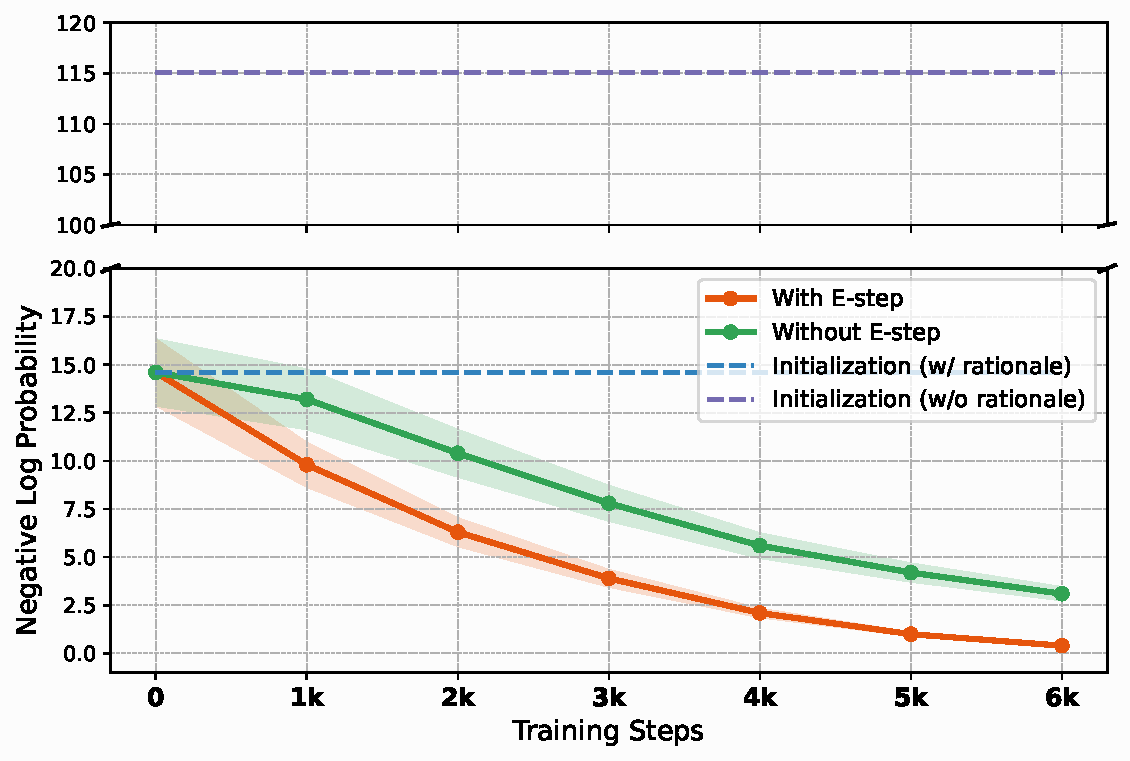
\includegraphics[width=0.75\linewidth]{em_nll_broken_axis.pdf}
    \caption{NLL trajectories during EM optimization.  
    Curves compare training \emph{with} and \emph{without} the E-step, alongside initialization references with and without rationales.  
    Confidence bands (shaded) are reported for the optimized variants.}
    \label{fig:em_nll}
\end{figure}
